\section{System and modeling choices}
\label{sec:system}

\begin{figure}[t]
\centering
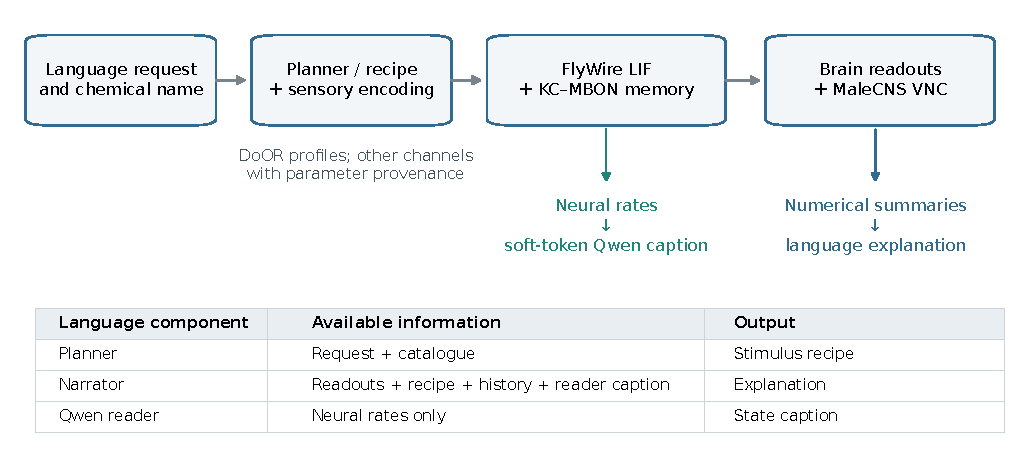
\includegraphics[width=\linewidth]{figures/fig1_system.pdf}
\caption{The platform connects an explicit stimulus recipe to neural dynamics, persistent memory, and recorded outputs. The three language roles have different information access: the planner selects actions, the narrator explains supplied records and can see the reader caption, and the frozen-Qwen reader receives a learned prefix derived only from neural rates. The fixed numerical case studies bypass language planning and execute recorded recipes directly.}
\label{fig:system}
\end{figure}
\subsection{Spiking brain and sensory inputs}
The core is a Brian2 leaky integrate-and-fire model using the FlyWire v783 graph and cell annotations \citep{dorkenwald2024,schlegel2024}. Our checkout contains 138,639 neurons. We build on the sensorimotor modeling approach of \citet{shiu2024}; the implementation and additional gain corrections are part of the present system rather than a new validation of all pathways. Between probes, membrane and synaptic-current states are reset. Learned synaptic factors can persist across probes.

For an identified chemical, the odor encoder maps available DoOR receptor responses to annotated glomerular sensory populations \citep{munch2016}. It subtracts the database spontaneous-response reference and clips negative values to zero, then averages receptor responses within a mapped glomerulus, omits responses below 0.05, and converts the remaining normalized values into Poisson drive using a configurable maximum rate, 150 Hz by default. These rates are an engineering conversion from normalized response data. Missing receptor measurements are not evidence of no response. An everyday object name takes a different route: a language resolver selects a chemical proxy from the available list. The chosen proxy and its coverage must therefore remain visible in the experiment record.

Other sensory channels target annotated populations with parameterized stimulation. Direct stimulation of looming-responsive projection neurons, for example, is not an image-to-retina visual model. We distinguish measured input profiles, anatomical or literature-based targeting, and engineering choices in Table~\ref{tab:provenance}.
\begin{table}[t]
\caption{Origin and interpretation of the main system components. Empirical input does not make every subsequent transformation empirically calibrated.}
\label{tab:provenance}
\small
\begin{tabularx}{\linewidth}{@{}p{0.20\linewidth}XX@{}}
\toprule
Component & Data or literature constraint & Implementation choice / scope \\
\midrule
Brain graph & FlyWire v783 connectivity and cell annotations & LIF dynamics; global parameters and selected gain/sign corrections \\
Chemical input & DoOR receptor-response profiles & Glomerular averaging, response threshold, rate scaling; partial coverage \\
Other senses & Annotated target populations and pathway literature & Stimulus-to-rate mapping; some inputs bypass peripheral processing \\
Plastic memory & KC--MBON/DAN anatomy and plasticity literature & Rate-based depression, threshold and floor; no explicit weight recovery \\
Motor bridge & MaleCNS v1.0 subgraph and motor annotations & Type/side matching, Poisson rate transfer; hybrid female/male assembly \\
Language interface & User text and recorded model state & Planner and narrator prompts; learned reader prefix; separate access to evidence \\
\bottomrule
\end{tabularx}
\end{table}


\subsection{Persistent plastic state}
The memory module maintains a multiplicative factor for each Kenyon-cell-to-mushroom-body-output-neuron (KC--MBON) connection. For an active synapse, a normalized KC rate and an MBON-specific dopamine signal produce a bounded multiplicative depression:
\begin{equation}
 m_{ij}^{\mathrm{new}}=\max\{m_{\min},\;m_{ij}(1-\eta a_i d_j)\}.
\end{equation}
Here $a_i$ is clipped KC activity and $d_j$ aggregates activity in dopamine neurons connected to the MBON, using connectivity-derived weights and a threshold. The rule is motivated by dopamine-dependent plasticity at mushroom-body output synapses \citep{hige2015}; the rate normalization, threshold, learning rate, and floor are implementation choices. Updates use mean rates over a completed probe rather than continuous spike timing; the caller controls when the rule is applied. The module saves the factors together with synapse indices. This implements persistent, experience-dependent weights; a learning claim additionally requires a changed output on matched probes. The rule has no explicit recovery term for depressed synapses, so opposite histories in separate models do not establish reversal learning in one model.

\subsection{Descending activity and motor outputs}
The motor bridge averages FlyWire descending-neuron rates by cell type and side and uses matched MaleCNS types as Poisson drivers for a ventral nerve cord (VNC) subgraph \citep{malecns2026}. The current construction has 1,314 descending drivers and 22,812 VNC neurons, including 708 annotated motor neurons. This joins a female brain reconstruction to a male CNS-derived subgraph. Type matching is a practical interface assumption, not a reconstruction of a single animal's nervous system. The output is motor-neuron activity. No biomechanical body, muscle dynamics, or movement-derived sensory feedback is implemented in this bridge.

\subsection{Three language roles}
The planner converts a user request into a structured stimulus plan. The narrator receives the accepted recipe, simulation summaries, history, memory information, and the reader caption and explains them. A separate soft-token reader maps a neural-rate vector into a frozen language model. These components have different information access and require different evaluations. Narrator statements cannot establish decoding from neural activity alone. Conversely, reader caption accuracy does not establish that the planner applied the intended physical stimulus.

The case-study records contain the recipe, actual neural inputs, seeds, sparse activity, memory state, and outputs. A manifest identifies source files, data dependencies, parameters, and active components. The numerical panels require their stated components; language roles are evaluated separately. The public-facing animation is a visualization of model outputs and does not add physiological evidence.
